\chapter{Evaluación y resultados}
\label{sec:Usuarios}

Para validar que la herramienta cumple con los objetivos planteados se ha llevado a cabo el plan de usuarios descrito a continuación.

\section{Pruebas con usuarios}
\label{sec:Pruebas}
Como se ha mencionado en la sección \ref{sec:Objetivos}, lo que se busca en este trabajo es una herramienta capaz de generar de manera similar a los humanos un árbol de comportamiento funcional o, al menos, una aproximación que sea capaz de disminuir el trabajo a los diseñadores de videojuegos.
Con este objetivo en mente se ha diseñado unas pruebas con usuarios para comprobar si se cumplen los objetivos planteados.

Para ello se ha realizado un plan de pruebas donde se evaluan los tiempos de ejecución de generación y ejecución de los árboles de comportamiento, la comparación entre los tiempos de un árbol generado por un humano y uno generado por la herramienta, los intentos de generación de un árbol y la calidad de la herramienta en cuanto a usabilidad y funcionalidad.
Para estas métricas las hipótesis iniciales eran las siguientes:
\begin{itemize}
    \item \texttt{H1}: La herramienta es capaz de generar árboles más rápido que un diseñador que los hace a mano
    \item \texttt{H2}: Los árboles generados realizan una ejecución similar a los realizados por un humano
    \item \texttt{H3}: La calidad de los árboles generados por la herramienta es un poco menor que los generados por un humano, pero les permite a los diseñadores tener un punto de partida más rápido que puede ser fácilmente modificable, disminuyendo así el tiempo de trabajo
    \item \texttt{H4}: La herramienta de generación de árboles es intuitiva y fácilmente de utilizar.
\end{itemize}

Para poder comprobar estas hipótesis se han buscado usuarios que cumplan con el perfil de un diseñador de videojuegos que haya trabajado con Unreal Engine y sus árboles de comportamiento.
El procedimiento con los usuarios ha sido el siguiente:
\begin{enumerate}
    \item Con el fin de mantener el anonimato, se le asigna un identificador único a cada usuario.
    \item Se le pide que haga un árbol de un NPC que patrulla hasta que ver a un objetivo, que debe perseguirlo hasta estar lo suficientemente cerca como para atacarlo.
    \item Se le pide que haga un árbol de un NPC que va recogiendo flores hasta que ve a un objetivo, que en ese caso debe huir a un punto del mapa.
    \item Se les cronometra desde el momento en el que se les indique que pueden empezar hasta que consigan una ejecución que satisfaga a los objetivos propuestos.
    \item Se les pide que realicen los mismos árboles con la herramienta.
    \item Se les pide que rellenen un formulario sobre la usabilidad y calidad de la herramienta.
\end{enumerate}

Para cada árbol que debería ser creado se hicieron dos escenarios distintos, uno en el que se deba usar la herramienta y otro en la que el NPC ejecuta un árbol creado a mano a través del sistema de Blueprints (sistema de programación visual de Unreal).
Para el primer árbol se ha hecho una copia del tercer escenario mencionado en la sección \ref{sec:Validacion}, con un objetivo y un punto de patrulla cerca de él en el mapa.
El segundo escenario consta de un objetivo, dos flores rojas (una de ellas en frente el objetivo para que el NPC tenga que pasar por delante de él) y un punto de patrulla alejado del objetivo.

El formulario, que se puede encontrar en el apéndice \ref{appendix:formularioUsuarios}, mide la usabiliad y la calidad de la herramienta frente a BTs creados por un humano.
Para la usabilidad se ha decidido evaluar mediante el System Usability Scale (SUS), que consiste en un cuestionario estandarizado de 10 items que siguen la escala de Likert de 5 puntos, que van desde ``Totalmente en desacuerdo'' a ``Totalmente de acuerdo'' (\cite{sus}).
Este método de evaluación se ha decidido seguir por evidencias de su robustez (\cite{Bangor} y \cite{ValSUS}).

Para la calidad de la herramienta se les han realizado preguntas sobre los resultados esperados de tiempos de ejecución, diferencias entre la calidad y similitud de sus árboles de comportamiento y los generados por la herramienta, y su funcionalidad como punto de partida.
Finalmente se ha habilitado un campo de texto no obligatorio de respuestas libres donde los usuarios podrían expresar su opinión sobre los árboles generados y la herramienta.

\section{Resultados de las pruebas de usuario}
\label{sec:Resultados}

Debido al perfil específico que se necesitaban para las pruebas solo se han podido realizar pruebas con 3 usuarios, por lo que las conclusiones sirven como una aproximación pero no se deben tomar como concluyentes.

\subsection{Resultados de la usabilidad de la herramienta}

En cuanto a la usabilidad podemos ver los resultados individuales en la tabla \ref{tab:sus} y en la figura \ref{fig:ResSUS} que se ha obtenido una media de 90.83 sobre 100 con una desviación estándar de 15.88, lo cual supera con creces la media de 68 establecida en la literatura, por lo que dadas estas pruebas se puede decir que la herramienta cumple con el objetivo de accesibilidad, haciéndola así fácil de utilizar y confirmando con los datos dados H4 (\cite{SUSRes}).

\begin{longtblr}[
    caption = {Resultados de la encuesta SUS},
    label = {tab:sus}
]{
colspec={|l|l|},
rowhead=1,
hlines,
row{even}={gray9},
cells   = {font=\footnotesize\linespread{0.84}\selectfont},
}
    \hline
    Usuario    & Puntuación \\  \hline
    U1    & 72.5   \\
    U2    & 100   \\
    U3  & 100   \\ \hline
\end{longtblr}

\begin{figure}[H]
    \centering
    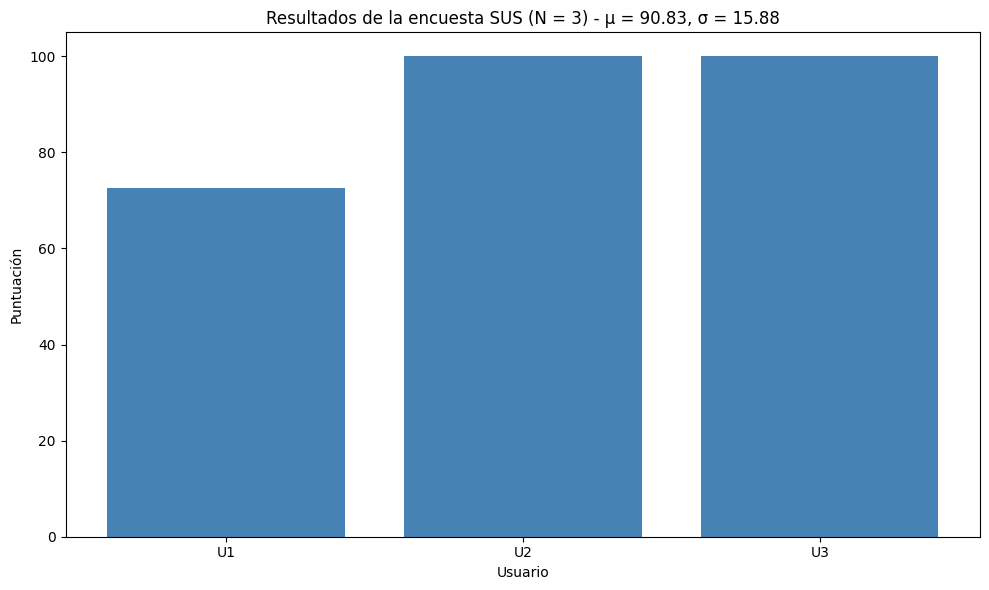
\includegraphics[width=1\textwidth]{Imagenes/Bitmap/ResultadosSUS.png}
    \caption[Resultados de la encuesta SUS]{Resultados de la encuesta SUS de los usuarios sobre la usabilidad de la herramienta.}
    \label{fig:ResSUS}
\end{figure}

\subsection{Resultado de la comparativa de tiempos}

La comparativa de los tiempos podemos verla en la tabla \ref{tab:CompTemp} y en la figura \ref{fig:CompTemp}, en donde a excepción del primer árbol de comportamiento que ha tardado más en generarlo la herramienta que el segundo usuario, hay una diferencia significativa en cuanto a la tardanza, beneficiando a los generados por la herramienta.
Además, como podemos ver en la figura \ref{fig:OpTemp}, los usuarios tienen una opinión favorable sobre los tiempos de ejecución de la herramienta con una media del 86.6\% y una desviación típica de 0.58, afirmando así la hipótesis inicial de generar de forma más rápida los árboles de comportamiento con unos tiempos de generación adecuados (H1).

\begin{longtblr}[
    caption = {Tiempo (en segundos) de generación de cada árbol de comportamiento por cada usuario},
    label = {tab:CompTemp}
]{
colspec={|l|l|l|l|l|},
rowhead=1,
hlines,
row{even}={gray9},
cells   = {font=\footnotesize\linespread{0.84}\selectfont},
}
    \hline
    Usuario    & Árbol 1 manual & Árbol 1 herramienta & Árbol 2 manual & Árbol 2 herramienta \\ \hline
    U1    & 578 & 238   & 332   & 142   \\
    U2    & 315 & 486   & 159   & 35   \\
    U3  & 271   & 35    & 174   & 37   \\ \hline
\end{longtblr}

\begin{figure}[H]
    \centering
    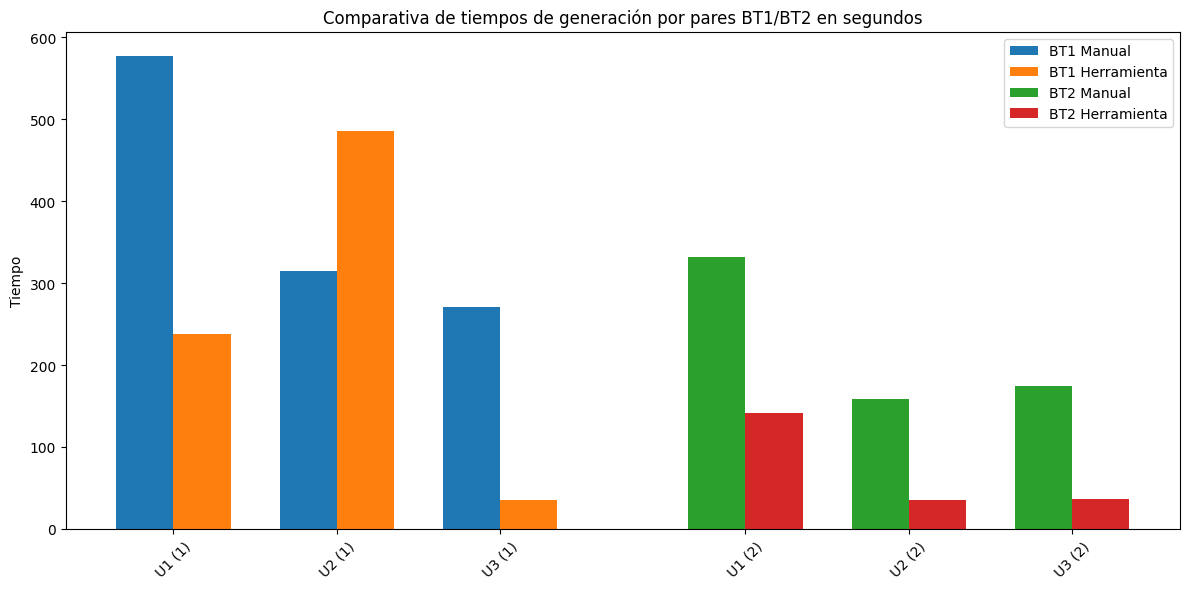
\includegraphics[width=1\textwidth]{Imagenes/Bitmap/ComparacionTiempos.png}
    \caption[Comparación de los tiempos de generación de los árboles de comportamiento]{Comparación de cuánto han tardado en crear los usuarios los árboles de comportamiento junto a cuánto ha tardado la herramienta.}
    \label{fig:CompTemp}
\end{figure}

\begin{figure}[H]
    \centering
    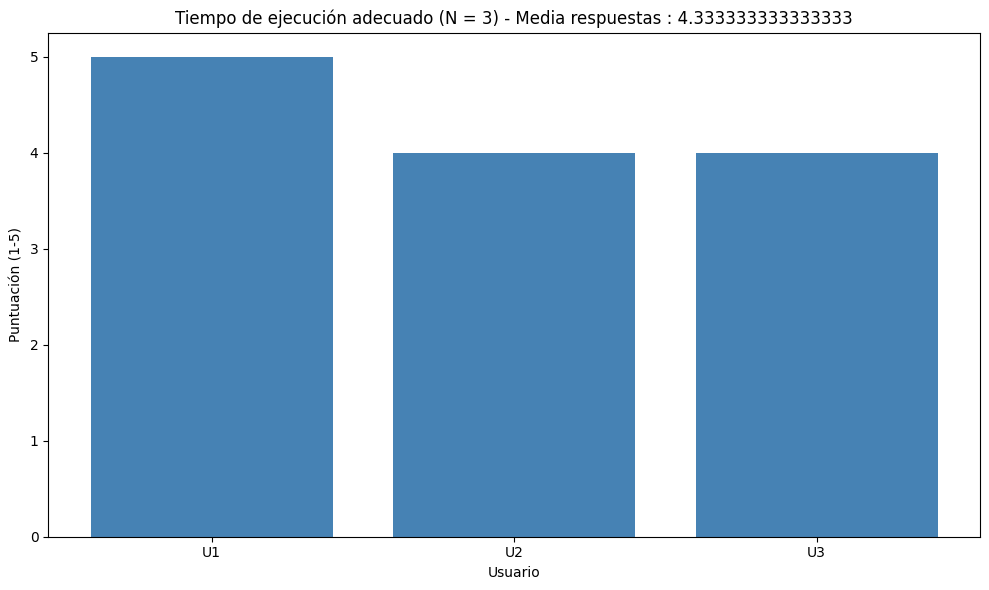
\includegraphics[width=1\textwidth]{Imagenes/Bitmap/OpinionTiempos.png}
    \caption[Opinión de los usuarios sobre los tiempos de generación de los árboles de comportamiento]{Opinión de los usuarios sobre los tiempos de ejecución de la herramienta generadora de árboles de comportamiento del 1 al 5, siendo 1 una opinión desfavorable y 5 la más favorable.}
    \label{fig:OpTemp}
\end{figure}

\subsection{Resultados de la calidad y disminución de carga de trabajo}

Siguiendo con la calidad de los árboles de comportamiento, podemos observar en las figuras \ref{fig:Calidad} y \ref{fig:Ejecucion} que la calidad de los árboles es inferior a los generados por un humano (con una media en las respustas del 80\% y una desviación típica de 1), pero que cumplen con la ejecución esperada (con una media de las respuestas del 80\% y una desviación típica de 0).
Esto se puede explicar gracias a las respuestas de las preguntas sobre si los árboles generados tenían más nodos de los necesarios y si eran distintos a los generados por los humanos, en los que todos los usuarios respondieron que la herramienta añadía algunos nodos extra (tanto compuestos como tareas innecesarias) y que esto hacía que los árboles generados fuesen distintos a los creados manualmente, dando una calidad inferior pero con una ejecución similar, confirmando así la hipótesis H2.

\begin{figure}[H]
    \centering
    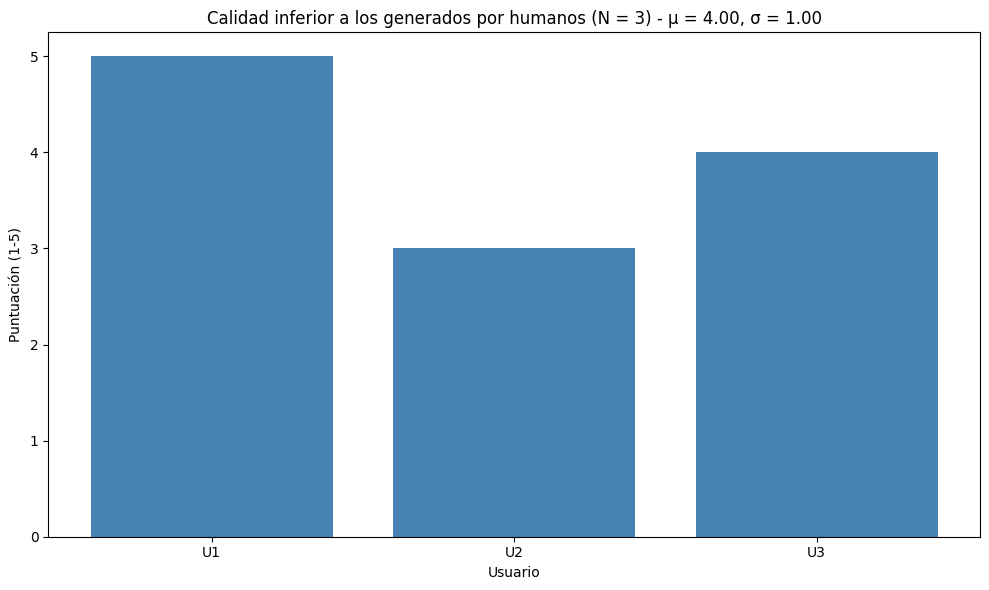
\includegraphics[width=1\textwidth]{Imagenes/Bitmap/CalidadInferior.png}
    \caption[Opinión de la calidad de los árboles de comportamiento]{Respuestas de los usuarios sobre la calidad de los árboles de comportamiento generados por la herramienta, donde 1 es que no están de acuerdo con la afirmación de que la calidad de los árboles generados por la herramienta son inferiores y 5 es que están completamente de acuerdo.}
    \label{fig:Calidad}
\end{figure}

\begin{figure}[H]
    \centering
    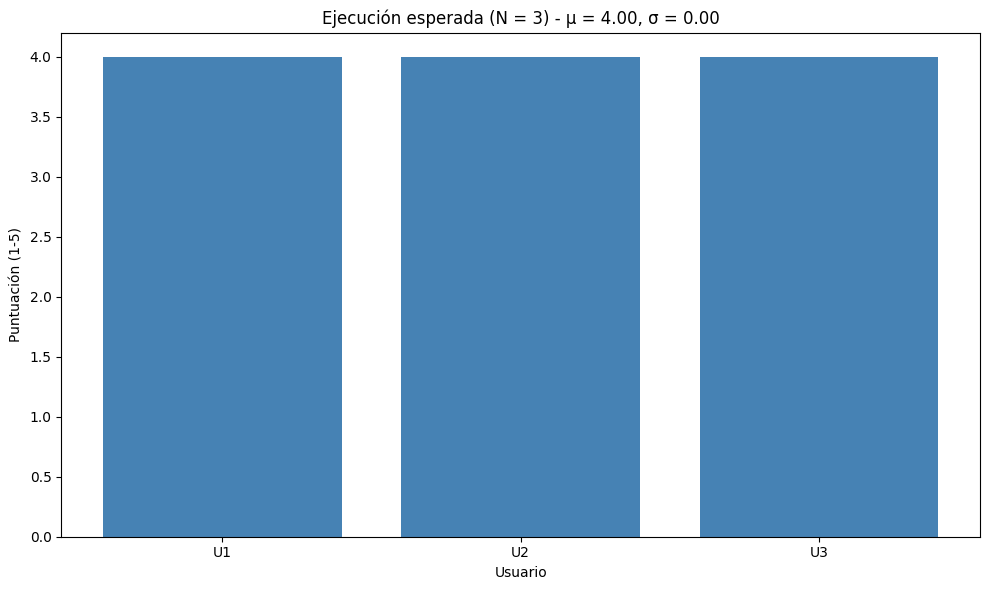
\includegraphics[width=1\textwidth]{Imagenes/Bitmap/EjecucionEsperada.png}
    \caption[Opinión de los usuarios sobre la ejecución esperada de los árboles de comportamiento]{Respuestas de los usuarios sobre la ejecución esperada de los árboles de comportamiento, donde 1 es que consideran una mala ejecución y 5 significa una ejecución correcta.}
    \label{fig:Ejecucion}
\end{figure}

Finalmente y junto a los resultados del apartado de calidad, la comprobación de H3 se puede apoyar en los resultados de las figuras \ref{fig:PtoPartida}, \ref{fig:Mod} y \ref{fig:Carga}, donde podemos ver que los usuarios han tenido una buena opinión sobre la idea de la usabilidad de la herramienta como apoyo para los diseñadores, respondiendo con un 93.4\% de media y una desviación típica de 0.58 a la opinión de que sirve como buen punto de partida y que, gracias a la facilidad de modificación de los JSONs generados (con una media de respuestas del 86.6\% y una desviación típica de 1.15), la herramienta puede servir para disminuir la carga de trabajo de los diseñadores (con una opinión de media del 93.4\% y una desviación típica de 0.58).

\begin{figure}[H]
    \centering
    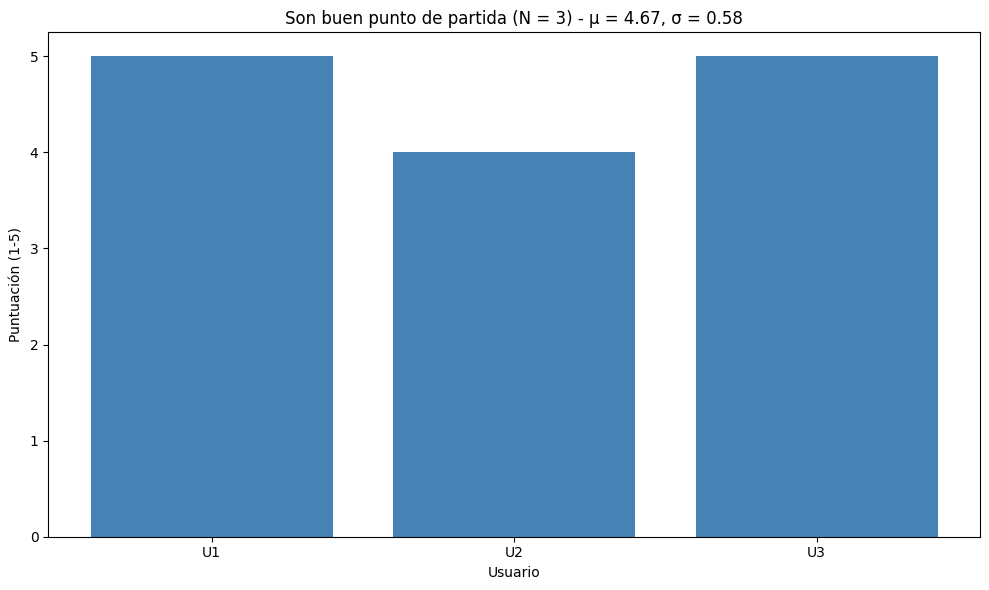
\includegraphics[width=1\textwidth]{Imagenes/Bitmap/PuntoDePartida.png}
    \caption[Opinión sobre si los árboles de comportamiento son un buen punto de partida]{Respuestas de los usuarios donde indican si los árboles de comportamiento generados sirven como punto de partida (5) o no (1)}
    \label{fig:PtoPartida}
\end{figure}

\begin{figure}[H]
    \centering
    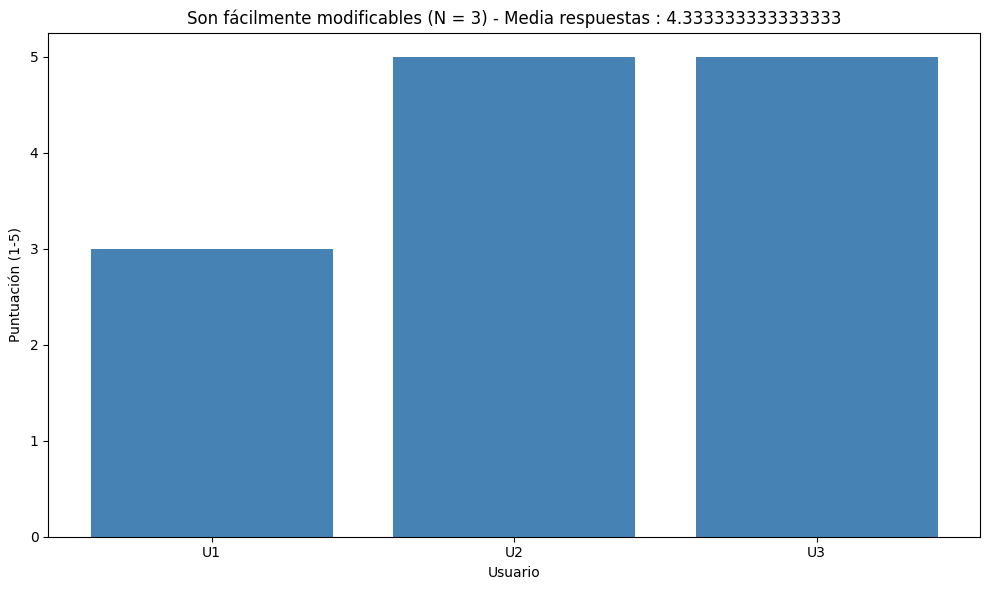
\includegraphics[width=1\textwidth]{Imagenes/Bitmap/Modificables.png}
    \caption[Opinión de los usuarios sobre si los resultados del árbol de comportamiento generado son fácilmente modificables]{Respuestas de los usuarios sobre la facilidad para modificar los árboles de comportamiento generados, donde 1 es significa que es dificil y 5 significa que es fácil.}
    \label{fig:Mod}
\end{figure}

\begin{figure}[H]
    \centering
    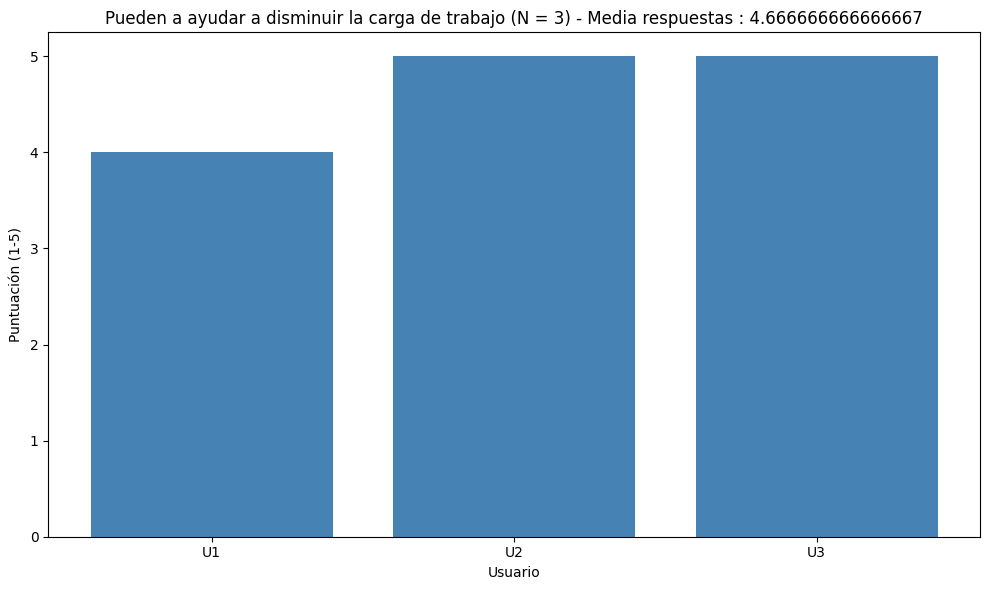
\includegraphics[width=1\textwidth]{Imagenes/Bitmap/CargaTrabajo.png}
    \caption[Opinión de los usuarios sobre si el uso de la herramienta disminuye la carga de trabajo de los diseñadores.]{Respuestas de los usuarios sobre su opinión de si la herramienta puede disminuir (5) o no (1) la carga de trabajo de los diseñadores.}
    \label{fig:Carga}
\end{figure}